%\section{Intro to Automated Formal Synthesis Optimization}
This Chapter presents the case studies used to evaluate the proposed approach of optimal sizing of stand-alone solar PV systems using automated synthesis. 
Moreover, the approach is compared with a simulation tool, named HOME Pro. 
The version and command-line of each verifier adopted, 
the computing setup, the objectives of the experimental phase, 
and the results itself are also described.

%---------------------------------------------------------------------------
\section{Optimization Case studies} 
%---------------------------------------------------------------------------

It was performed seven stand-alone PV system case studies to evaluate the proposed synthesis approach: 

\begin{itemize}
\item Case Study 1: Power peak: 342 W, power surge: 342 W, energy consumption: 3,900 Wh/day, battery autonomy: 48 h;
\item Case Study 2: Power peak: 814 W, power surge: 980 W, energy consumption: 4,880 Wh/day, battery autonomy: 48 h;
\item Case Study 3: Power peak: 815 W, power surge: 980 W, energy consumption: 4,880 Wh/day, battery autonomy: 12 h;
\item Case Study 4: Power peak: 253 W, power surge: 722 W, energy consumption: 3,600 Wh/day, battery autonomy: 48 h;
\item Case Study 5: Power peak: 263 W, power surge: 732 W, energy consumption: 2,500 Wh/day, battery autonomy: 48 h;
\item Case Study 6: Power peak: 322 W, power surge: 896 W, energy consumption: 4,300 Wh/day, battery autonomy: 48 h;
\item Case Study 7: Power peak: 1,586 W, power surge: 2,900 W, energy consumtion: 14,000 Wh/day, battery autonomy: 48h.
\end{itemize}

These case studies were defined based on usual electrical load found in riverside communities of the Amazon State in Brazil~\cite{abs-1811-09438, Agrener2013}. With exception of case 7 that was idealized as a small town solution to support few lamps and an 12 kBTUs air-conditioner.

%---------------------------------------------------------------------------
\section{Objectives and Setup} 
%---------------------------------------------------------------------------

The evaluation aims to answer two experimental questions: 

\begin{enumerate}

\item[EQ1] \textbf{(soundness)} does the proposed automated synthesis approach provide correct results?

\item[EQ2] \textbf{(performance)} how do the software verifiers compare to each other?

\end{enumerate}

All experiments regarding the verification tools were conducted 
on an otherwise idle Intel Xeon CPU E5-4617 ($8$-cores) with 
$2.90$ GHz and $64$ GB of RAM, running Ubuntu $16.04$ LTS $64$-bits. 
Related to HOMER Pro, it was used an Intel Core i5-$4210$ ($4$-cores), 
with $1.7$ GHz and $4$ GB of RAM, running Windows 10. 
The experiments were performed with a predefined time out of $240$ minutes.

Three start-of-art verification tools, CBMC\footnote{Command-line: \$ cbmc -\phantom{}-unwind 100 filename.c -\phantom{}-trace} version 5.11 with MiniSat 2.2.1~\cite{Kroening}, ESBMC\footnote{Command-line: \$ esbmc filename.c -\phantom{}-no-bounds-check -\phantom{}-no-pointer-check -\phantom{}-unwind 100 -\phantom{}-boolector} version 6.0.0 with solver Boolector 3.0.1~\cite{Brummayer}, %UAutomizer\footnote{Command-line: \$ ./Ultimate -tc config/AutomizerReach.xml -s config/svcomp-Reach-32bit-Automizer\_Default.epf -i filename.c -\phantom{}-traceabstraction.limit.analysis.time 900 -\phantom{}-traceabstraction.stop.after.first.violation.was.found false -\phantom{}-cacsl2boogietranslator.overapproximate.operations.on.floating.types false -\phantom{}- cacsl2boogietranslator.assume.nondeterminstic.values.are.in.range false -\phantom{}-rcfgbuilder.add.additional.assume.for.each.assert true -\phantom{}-rcfgbuilder.simplify.code.blocks true -\phantom{}-rcfgbuilder.size.of.a.code.block LoopFreeBlock}, 
and CPAchecker\footnote{Command-line: \$ scripts/cpa.sh -heap 64000m -config config/bmc-incremental.properties -spec config/specification/sv-comp-reachability.spc filename.c} version 1.8 with MathSAT 5.5.3~\cite{mathsat5}, were used as verification engine to compare the proposed approach effectiveness and efficiency. Note that ``incremental'' ESBMC with the SMT solver Z3 version 4.7.1~\cite{DeMoura} was tried\footnote{Command-line: \$ esbmc filename.c -\phantom{}-no-bounds-check -\phantom{}-no-pointer-check -\phantom{}-unwind 100 -\phantom{}-smt-during-symex -\phantom{}-smt-symex-guard -\phantom{}-z3} as an alternative to use less computing memory. The Simulation tool HOMER Pro version $3.13.1$ was used for comparative purpose.

%---------------------------------------------------------------------------
\section{Results}  
\label{sec:synthesisresults}
%---------------------------------------------------------------------------

The results are presented at Table~\ref{tab1}. 

\begin{table}
\caption{Case studies and results: optimization of stand-alone PV systems.}\label{tab1}
\begin{scriptsize}
\begin{tabular}{|c|c|c|c|c|}
\hline
\hline
Tools & \makecell{CBMC 5.11 \\(MiniSat 2.2.1)}& \makecell{ESBMC 6.0.0 \\(Boolector 3.0.1 /\\Z3 4.7.1)}& \makecell{CPAchecker 1.8\\(MathSAT 5.5.3)}& HOMER Pro 3.13.1\\
\hline
\hline
Specification & Result & Result & Result & Result \\
\hline
\makecell{\textbf{Case Study 1}\\Peak:342W\\Surge:342W \\E:3,900Wh/day\\Autonomy:48h} & OM & TO / IF & \makecell{SAT (172.03 min) \\NTP:1$\times$340W (1S)\\NBT:8$\times$105Ah (2S-4P)\\Controller 15A/75V\\Inverter 700W/48V\\LCC: US\$ 7,790.53} & \makecell{(Time: 0.33 min)\\2.53 kW of PV\\NBT:12$\times$83.4Ah (2S-6P)\\0.351kW inverter\\LCC: US\$ 7,808.04}\\
\hline
\makecell{\textbf{Case Study 2}\\Peak:814W\\Surge:980W\\E:4,880Wh/day\\Autonomy:48h} & OM & TO / IF & \makecell {SAT (228.7 min) \\NTP:2$\times$330W (2S)\\NBT:10$\times$105Ah (2S-5P)\\Controller 20A/100V DC\\Inverter 1,200W/24V \\LCC: US\$ 8,335.90} & \makecell{(Time: 0.18 min)\\3.71 kW of PV\\NBT:20$\times$83.4Ah (2S-10P)\\0.817kW inverter\\LCC: US\$ 12,861.75} \\
\hline
\makecell{\textbf{Case Study 3}\\Peak:815W\\Surge:980W\\E:4,880Wh/day\\Autonomy:12h} & OM & TO / IF & \makecell {SAT (166.13 min) \\NTP:4$\times$150W (4S)\\NBT:4$\times$80Ah (2S-2P)\\Controller 15A/100V DC\\Inverter 1,200W/24V \\LCC: US\$ 7,306.27} & Not possible \\
\hline
\makecell{\textbf{Case Study 4}\\Peak:253W\\Surge:722W\\E:3,600Wh/day\\Autonomy:48h} & OM & TO / IF & \makecell {SAT (143.71 min) \\NTP:4$\times$150W (4S)\\NBT:10$\times$80Ah (2S-5P)\\Controller 15A/75V\\Inverter 750W/24V \\LCC: US\$ 7,816.31} & \makecell{(Time: 0.23 min)\\2.42 kW of PV\\NBT:12$\times$83.4Ah (2S-6P)\\0.254kW inverter\\LCC: US\$ 7,677.95}\\
\hline
\makecell{\textbf{Case Study 5}\\Peak:263W\\Surge:732W\\E:2,500Wh/day\\Autonomy:48h} & OM & TO / IF & \makecell {SAT (134.93 min) \\NTP:1$\times$340W (1S)\\NBT:6$\times$105Ah (2S-3P)\\Controller 15A/75V\\Inverter 400W/24V \\LCC: US\$ 7,252.14} & \makecell{(Time: 0.18 min)\\1.59 kW of PV\\NBT:10$\times$83.4Ah (2S-5P)\\0.268kW inverter\\LCC: US\$ 6,175.57} \\
\hline
\makecell{\textbf{Case Study 6}\\Peak:322W\\Surge:896W\\E:4,300Wh/day\\Autonomy:48h} & OM & TO / IF & \makecell {SAT (235.75 min) \\NTP:2$\times$200W (2S)\\NBT:10$\times$105Ah (2S-5P)\\Controller 15A/75V\\Inverter 400W/24V \\LCC: US\$ 8,287.23} & \makecell{(Time: 0.22 min)\\3.15 kW of PV\\NBT:14$\times$83.4Ah (2S-7P)\\0.328kW inverter\\LCC: US\$ 9,112.45} \\
\hline
\makecell{\textbf{Case Study 7}\\Peak:1,586W\\Surge:2,900W\\E:14,000Wh/day\\Autonomy:48h} & OM & TO / IF & TO & \makecell{(Time: 0.20 min)\\12.5 kW of PV\\NBT:66$\times$83.4Ah (2S-33P)\\1.60kW inverter\\LCC: US\$ 41,878.11} \\
\hline
\hline
\end{tabular}
\\Legend: OM = out of memory; TO = time out; IF = internal failure, E = energy.
\end{scriptsize}
\end{table}

CPAchecker was able to synthesize the optimal sizing in six 
out of seven case studies (cases $1$ to $6$): the result was produced within 
the time limit, which varied from $134.71$ to $235.75$ minutes. Fig.~\ref{fig:CPAoptc1} illustrates the result of case 4 with the optimal sizing appearing in the left size as the integer $8$ to the solar panel (which is the model RSM36-6-150P from manufacturer Risen), battery $0$ that means the model 12MF80 of 80 Ah from Moura, charge controller $1$ that means the model 15A-75V MPPT from Victron  Energy, and the inverter number $3$ means the model IP350-11 from Epever (750 W). The variables NTP, NPS, NPP, NPS, NBP, and NBTotal, presented at the counter-example as well, shows how many and how the panels and batteries are connected.

Only case study $7$ led to a \textit{time out} result in CPAchecker, i.e., 
it was not solved within $240$ minutes. However, if it is removed 
this time out limitation from CPAchecker, the verifier is 
able to solve the optimization in $44.97$ hours. 
The violation (SAT result) indicated in Table~\ref{tab1} 
is the $assert$ of line $22$ from Algorithm~\ref{alg:verification-algorithm}. %The results were tested by manual PV sizing and were sound (\textit{RQ1}). %, linking a feasible technical solution with the lowest cost possible, considering the equipment that were inputted to the code. 

\begin{figure}[h]
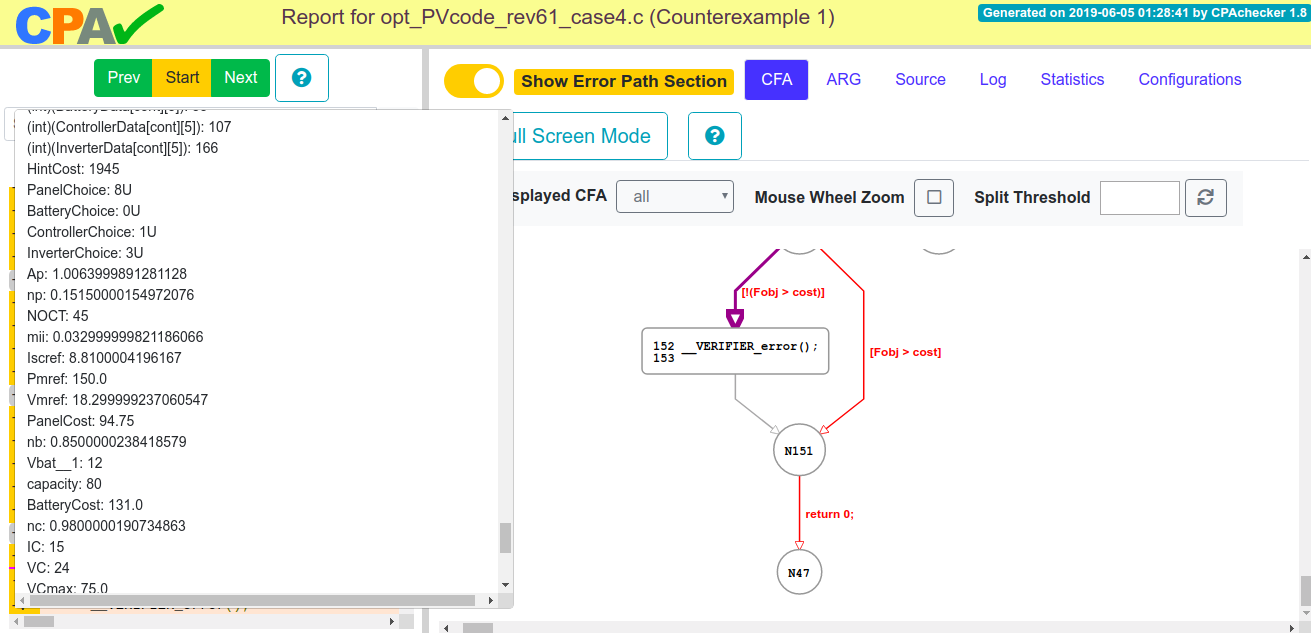
\includegraphics[width=1.0\textwidth]{CPA_opt_c4.png}
\centering
\caption{Counter-example generated by CPAchecker after validation of case 4 (file Counterexample.html).}
\label{fig:CPAoptc1}
\end{figure}

CBMC and ESBMC are unable to produce any conclusive result. 
Situations of \textit{internal failure}, \textit{time out}, 
or \textit{out of memory} occurred; this partially answers 
the \textit{EQ2}. Note that the internal failure presented 
by ESBMC was a Z3 solver issue (a bug); this will demand 
an updated version of ESBMC to fix this issue. Similarly to CPAchecker, 
if it is removed the \textit{time out} from ESBMC with the SMT solver Boolector, 
then the verifier is able to obtain the automated synthesis 
in $73.18$ hours for the case study $2$. CBMC, in the other hand, only could present some result if the RAM memory of the system was bigger to avoid the \textit{memory out} issue.

Related to HOMER Pro, it was able to evaluate six case studies (cases $1$, $2$, $4$, $5$, $6$, and $7$), and within a time shorter than $30$ seconds, which was much 
faster than the proposed automated synthesis tool (cf.~\textit{EQ2}). 
Case study $3$ was not possible to be simulated since HOMER Pro 
does not have the feature of adjusting the battery autonomy, i.e., 
the tool always tries to feed with electricity the given load 
during $365$ days/year. 

Fig.~\ref{fig:homeroptc4} illustrates parts of the 9-page PDF report presented by HOMER Pro, specifically for the case 4.

\begin{figure}[h]
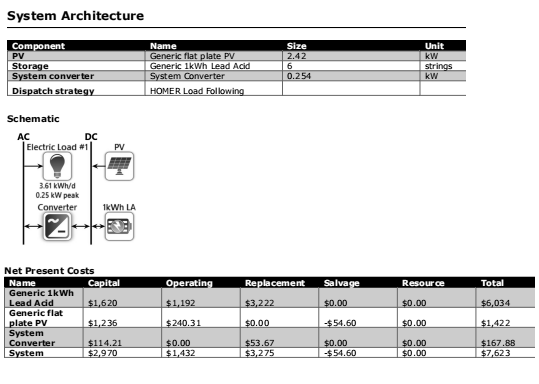
\includegraphics[width=0.8\textwidth]{homeroptc4.png}
\centering
\caption{Optimization report (partial) from HOMER Pro (case 4).}
\label{fig:homeroptc4}
\end{figure}

It was also noted other HOMER Pro drawbacks:

\begin{itemize}
\item There exists no explicit charge controller 
as a system equipment. HOMER Pro includes automatically 
a controller just to simulate the charge/discharge 
of batteries and to meet the load requirement; however, 
without costs or even with electrical characteristics 
as maximum current and voltage, which are common during PV sizing;
\item HOME Pro demands to include some battery specification 
to initiate the optimization; however, it does not change 
the electrical specifications during the simulation; 
the presented results are multiples of the original 
battery type suggested by the user. As example, it was 
started with a $83.4$ Ah lead-acid battery and during 
the simulation, HOMER Pro did not try to use other capacities or types;
\item HOMER Pro does not present the optimal solution 
in terms of connections of arrays of PV panels, just the 
total in terms of power, i.e., it does not present neither models 
and the power of each PV panel nor the total of panels in series or parallel. 
\end{itemize}

%%%%%%%%%%%%%%%%%%%%%%%%%%%%%%%%%%%%%%%%%%%%%%%%%%%%%%%%%%%%%%%%%%%%
\section{Comparison between Formal Synthesis and HOMER Pro}
%%%%%%%%%%%%%%%%%%%%%%%%%%%%%%%%%%%%%%%%%%%%%%%%%%%%%%%%%%%%%%%%%%%%

Comparing the results between the formal synthesis with CPAchecker 
and HOMER Pro, it was observed that most results are quite similar, 
in terms of technical solution and cost (cf. Table~\ref{tab1}). 

Particularly related to LCC, the cost was very close in cases 
$1$, $4$, $5$ and $6$, with difference varying from $0.23$\% to $17.4$\%. 
Even adopting the same price per kW to the PV panels, 
inverters, and batteries, HOMER Pro does not use costs 
related to charge controllers, which were introduced into the 
CPAchecker modeling. The premise used in CPAchecker to adopt 
a fixed annual cost for operation and maintenance can produce 
some impact as well at this discrepancy; however, it is not significant
since this annual cost is too small when compared to the resulting LCC value.

However, there exists a huge divergence in case study $2$, 
where the costs presented by HOMER Pro were $54$\% higher 
than the automated synthesis tool, probably because the 
operation and maintenance costs assumed by the automated 
synthesis tool were underestimated to that specific load. 

In general, the size of the PV panels and battery bank were 
bigger in HOMER Pro than with the formal synthesis approach, 
and that discrepancy is not easy to address without some real 
systems validation. The mathematical models are different and 
particular parameters can be tuned as well in each approach, 
and that can justify the difference, which was presented in all 
the case studies. As comparative, let's consider case study $1$: 
the optimal solution provided by HOMER Pro demands $7$ $\times$ 
more PV panels than the solution presented by the synthesis tool, 
and HOME Pro does not show the arrangement of arrays 
(i.e., the number of series and parallel PV panels); 
the battery bank presented by HOMER Pro provides $500.4$ Ah 
of capacity ($6 \times 83.4$), while the synthesis tool 
presented an optimal solution with $420$ Ah of total capacity 
($4 \times 105$). 

Just to compare the results obtained from the optimization 
with the real-world, the authors had four PV systems deployed 
and monitored since June $2018$ in a riverside community 
in the Amazonas State in Brazil, with similar demands 
presented by case studies $1$, $4$, $5$, and $6$, 
always with a $3$ $\times$ $325$ W ($3$S) panels and 
$4$ $\times$ $220$ Ah ($2$S-$2$P $= 440$ Ah) 
lead-acid batteries. These solutions are more close 
to the result presented by the proposed formal synthesis 
approach than HOMER Pro, thereby showing that the 
solution is sound, which answers \textit{EQ1}.

Related to the inverters, HOMER Pro suggests a value in 
kW very close to the peak of every case study, and it 
is just a reference value and not a commercial value of 
the employed inverter. The proposed synthesis tool, however, 
presents inverters that are commercial and can be found 
off-the-shelf. Therefore is a PRO to the formal synthesis method.

Concerning to charge controllers, as it was reported in 
the section~\ref{sec:synthesisresults}, HOMER Pro does not include it 
as an explicit equipment in its mathematical model, 
only the synthesis tool presents a commercial controller 
and includes it during the cost analysis. Therefore, 
the formal synthesis method presents more reliable results than
HOME Pro.

Case study $7$ was not solved by the synthesis tool 
within the time limit established during the experimental 
phase. Case study $3$ was not possible to simulate in HOMER Pro, 
because its restriction does not allow one to set the battery autonomy, 
thus resting both without parameters to comparative.

Summarizing, the synthesis tool is capable to present a 
solution, which is far detailed and close to the commercial 
reality than the solution presented by HOMER Pro. 
In particular, the automated synthesis method 
can provide all the details of every component of 
a PV system solution, with complete electrical details 
from data sheet of manufacturers, including 
the model of the component, nominal current and voltage. 
In this respect, even the name of the manufacturer 
can be presented (in Table~\ref{tab1} it was removed 
to avoid some advertising).
%used with the SMT incremental mode\footnote{Command-line: \$ esbmc filename.c -\phantom{}-no-bounds-check -\phantom{}-no-pointer-check -\phantom{}-unwind 100 -\phantom{}-smt-during-symex -\phantom{}-smt-symex-guard -\phantom{}-z3} enabled with the goal of reducing memory usage; we have also used the SMT solver Z3 version 4.7.1~\cite{DeMoura}.

%%%%%%%%%%%%%%%%%%%%%%%%%%%%%%%%%%%%%%%%%%
\section{Threats to validity}
%%%%%%%%%%%%%%%%%%%%%%%%%%%%%%%%%%%%%%%%%%

At this Section, it was reported a favorable assessment of proposed formal synthesis method. 
Nevertheless, it was also identified three threats to the validity 
of the experimental results, which can be further assessed and 
constitute future work: 

\begin{itemize}
\item ($1$) improvement of the power reliability 
analysis: to include loss of load probability or loss of power 
supply probability, which can make the analysis more accurate; 
\item ($2$) the cost analysis is well tailored to the Amazon region of Brazil; 
however, a broad analysis from other isolated areas must be 
performed in order to make the optimization general in terms 
of applicability; 
\item ($3$) to deploy at the field some PV systems 
sized using the synthesized results in order to validate it.
\end{itemize}


\section{Conclusion}

At this Chapter it was performed the comparative among verifiers with the proposed automated synthesis using model checking, in order to obtain the optimal sizing of stand-alone solar PV systems, which showed that CPAchecker had the best overall performance. CBMC and ESBMC were not conclusive for all the cases, reaching the \textit{time out} stipulated ($240$ minutes) or by \textit{out of memory} issue. CPAchecker was not possible to present a conclusive result just in case $7$ (\textit{time out}).

A comparative with a specialized simulation tool was performed as well, however in just $5$ case studies (case $1$, case $2$, case $4$, case $5$, and case $6$) it was possible comparative for the presented result. Some limitations of the simulation tool, mainly related to not allow battery autonomy setup, and the $time out$ or $out of memory$ messages presented by the verifiers, restricted the comparative between automated verification tools versus simulation tools. However, when the comparative was possible, it was noticed that the LCC was very close, and that HOMER Pro overestimated the sizing.

Based on the fact that mostly case studies were deployed at the field (case $1$, case $4$, case $5$, and case $6$), with regular visiting to perform interview with the dwellers, and with monitoring system in those houses, it was possible to compare the computer obtained results with the real world employment of the stand-alone solar PV systems. The final conclusion was that the proposed tool is sound, with an acceptable performance, and with a better quality of the presented output.